\begin{frame}
	\frametitle{Parameter tuning and control}
	
	\begin{figure}
		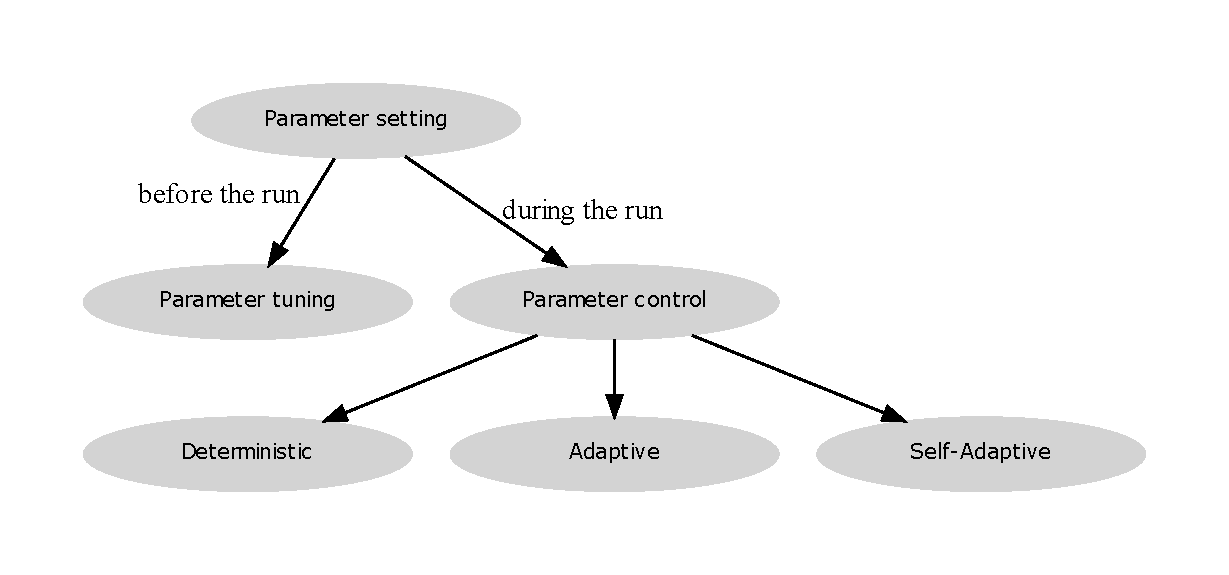
\includegraphics[width=0.9\textwidth]{figures/flowchart_parameter_control}
	\end{figure}
	\cite{Eiben.1999}
	
\end{frame}

\begin{frame}
	\frametitle{Length of Exploration Phase}
	
	\begin{columns}[c]
		
		\column{.45\textwidth}

		\begin{itemize}
			\item compare landscape features ever 10\%
			\item using Euclidean distance
			\item trade-off between
				\begin{itemize}
					\item time for exploration
					\item time for adjusted configuration
				\end{itemize}
			\item between 20 and 40\% from search (percentage of classification)
		\end{itemize}
		
		\column{.45\textwidth}
		\begin{figure}
			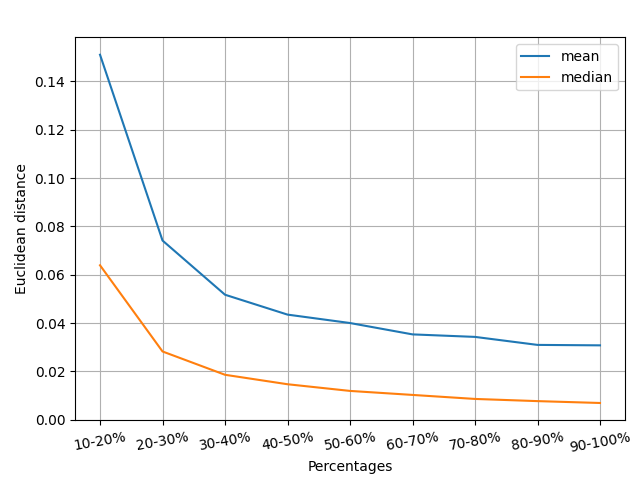
\includegraphics[width=1\textwidth]{figures/euclidean_distances}
		\end{figure}
		
		
	\end{columns}
	
\end{frame}

\begin{frame}
	\frametitle{Machine learning algorithm}
	
	\begin{itemize}
		\item binary classification
		\item supervised learning
		\item fast classification
		\item few features
		\item decision tree
	\end{itemize}
	
\end{frame}

\begin{frame}
	\frametitle{Hyper-parameter search}
	
	\begin{itemize}
		\item only apply on as many as possible
			\begin{itemize}
				\item TPR > 80\%
			\end{itemize}
		\item only apply if positive effect
			\begin{itemize}
				\item FPR < 5\%
			\end{itemize}
		\item percentage of classification (POC)
		\item construction criteria (Gini Impurity, Entropy or Log-Loss)
		\item depth of decision tree
	\end{itemize}
	
\end{frame}

\begin{frame}
	\frametitle{Influence on runtime}
	\begin{figure}
		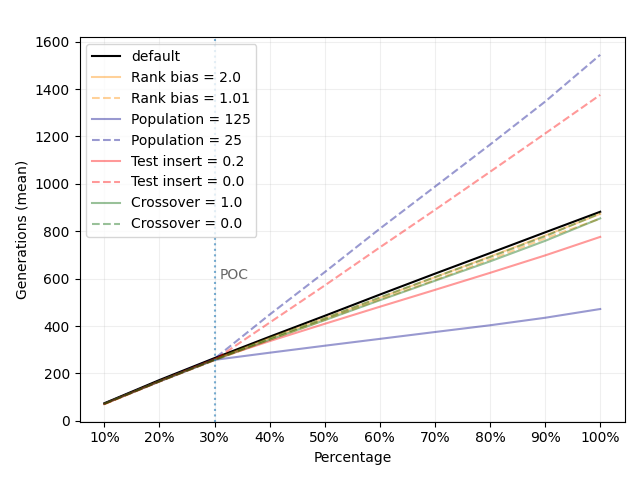
\includegraphics[height=0.9\textheight]{figures/generations_parameter}
	\end{figure}	
\end{frame}

\begin{frame}
	\frametitle{Event probability}
	
	\begin{columns}[c]
		
		\column{.35\textwidth}
		
		\begin{itemize}
			\item runtime in relation to event probability
			\begin{itemize}
				\item insert
				\item mutate
				\item crossover
			\end{itemize}
			\item trade-off
			\begin{itemize}
				\item fitness evaluation
				\item event occurrence
			\end{itemize}
		\end{itemize}
		
		\column{.60\textwidth}
		\begin{equation}
			P_{adj}(e) = \frac{n_1 P_1(e) + n_2 P_2(e)}{n_1 + n_2}
		\end{equation}
		
		\begin{equation}
			\hat{P}(e) = \sum_{i=k}^n \frac{n!}{i!(n-i)!} P_{adj}(e)^i (1-P_{adj}(e))^{n-i}
		\end{equation}
		
	\end{columns}
	
\end{frame}

\begin{frame}
	\frametitle{Parameter experiments}
	
	\begin{table}
		\centering
		\resizebox{\textwidth}{!}{\begin{tabular}{lll|lll|lll|ll}
\hline
                           &              &            & \multicolumn{3}{l|}{$P_{adj}$}                & \multicolumn{3}{l|}{$\hat{P}$ for $k = 5$}                 &            &            \\
configuration              & gen.         & n          & mut.          & cross.        & ins.          & mut.          & cross.          & ins.                     & $n\_+$       & $n\_-$       \\ \hline
default                    & 853          & 9          & 0.95          & 0.68          & 0.05          & 1.0           & 0.87            & 0.0                      &          &          \\
p = 25                     & 1,263        & 13         & 0.96          & 0.69          & 0.04          & 1.0           & 1.0 $\nearrow$  & 0.0                      & 0          & 0          \\
p = 125                    & 572          & 6          & 0.95          & 0.68          & 0.04          & 0.77          & 0.15            & 0.0                      & 3          & 0          \\
cr = 0.0                   & 841          & 8          & 0.95          & 0.0           & 0.05          & 1.0           & 0.0             & 0.0                      & 1          & 0          \\
cr = 1.0                   & 849          & 8          & 0.95          & 0.95          & 0.05          & 1.0           & 1.0 $\nearrow$  & 0.0                      & 0          & 0          \\
bias = 2.0                 & 912          & 9          & 0.95          & 0.68          & 0.05          & 1.0           & 0.88 $\nearrow$ & 0.0                      & 1          & 0          \\
bias = 1.01                & 824          & 8          & 0.95          & 0.68          & 0.05          & 1.0           & 0.77            & 0.0                      & 0          & 0          \\
pti = 0.0                  & 1,154        & 12         & 1.0           & 0.75          & 0.0           & 1.0           & 1.0 $\nearrow$  & 0.0                      & 0          & 4          \\
pti = 0.2                  & 770          & 8          & 0.92          & 0.63          & 0.08          & 1.0           & 0.66            & 0.0                      & 0          & 0          \\
p = 10, pti = 5.0          & 912          & 9          & 0.58          & 0.13          & 0.42          & 0.69          & 0.0             & 0.31 $\nearrow$          & 3          & 0          \\
\textbf{p = 25, pti = 1.0} & \textbf{777} & \textbf{8} & \textbf{0.75} & \textbf{0.38} & \textbf{0.25} & \textbf{0.89} & \textbf{0.14}   & \textbf{0.03 $\nearrow$} & \textbf{4} & \textbf{0} \\ \hline
\end{tabular}}
	\end{table}
	
\end{frame}

\begin{frame}
	\frametitle{Adaptive parameter control}
	
	\begin{columns}[c]
		
		\column{\textwidth}
		\blockheading{Known sample $S_1$}
			
		\begin{table}
			\centering
			\resizebox{\textwidth}{!}{\begin{tabular}{llllllll}
\hline
\multicolumn{1}{l|}{}                                                       & \multicolumn{2}{l|}{coverage DynaMOSA}               & \multicolumn{2}{l|}{coverage APC-DynaMOSA}                &                &                \\
\multicolumn{1}{l|}{CUT}                                                    & mean           & \multicolumn{1}{l|}{std}            & mean           & \multicolumn{1}{l|}{std}            & $\hat{A}_{12}$ & p-value     &    \\
\hline
\multicolumn{1}{l|}{\textbf{o.d.j.m.AbstractDBObject}}                      & \textbf{0.951} & \multicolumn{1}{l|}{\textbf{0.018}} & \textbf{0.960} & \multicolumn{1}{l|}{\textbf{0.039}} & \textbf{0.880} & \textbf{0.000} & $\nearrow$\\
\multicolumn{1}{l|}{\textbf{d.o.f.g.s.RoundStatsDiagram}}                   & \textbf{0.505} & \multicolumn{1}{l|}{\textbf{0.466}} & \textbf{0.000} & \multicolumn{1}{l|}{\textbf{0.000}} & \textbf{0.935} & \textbf{0.000} & $\searrow$\\
\multicolumn{1}{l|}{\textbf{c.a.a.c.d.t.u.i.p.DHTUDPPacketHandlerStats}}    & \textbf{0.909} & \multicolumn{1}{l|}{\textbf{0.010}} & \textbf{0.894} & \multicolumn{1}{l|}{\textbf{0.020}} & \textbf{0.917} & \textbf{0.001} & $\searrow$\\
\multicolumn{1}{l|}{\textbf{o.p.g.d.VisualPageListItem}}                    & \textbf{0.112} & \multicolumn{1}{l|}{\textbf{0.001}} & \textbf{0.113} & \multicolumn{1}{l|}{\textbf{0.002}} & \textbf{0.933} & \textbf{0.003} & $\nearrow$\\
\multicolumn{1}{l|}{\textbf{n.s.s.c.s.a.RollbackAction}}                    & \textbf{0.170} & \multicolumn{1}{l|}{\textbf{0.320}} & \textbf{0.000} & \multicolumn{1}{l|}{\textbf{0.000}} & \textbf{0.935} & \textbf{0.006} & $\searrow$\\
\multicolumn{1}{l|}{\textbf{f.v.n.m.b.s.p.w.p.GetParametersForm}}           & \textbf{0.111} & \multicolumn{1}{l|}{\textbf{0.152}} & \textbf{0.219} & \multicolumn{1}{l|}{\textbf{0.146}} & \textbf{0.935} & \textbf{0.008} & $\nearrow$\\
\multicolumn{1}{l|}{\textbf{d.h.l.e.i.e.AbstractMessageBasedEventProducer}} & \textbf{0.426} & \multicolumn{1}{l|}{\textbf{0.018}} & \textbf{0.439} & \multicolumn{1}{l|}{\textbf{0.023}} & \textbf{0.913} & \textbf{0.020} & $\nearrow$\\
\multicolumn{1}{l|}{\textbf{c.i.s.LocalFileBrowser}}                        & \textbf{0.126} & \multicolumn{1}{l|}{\textbf{0.128}} & \textbf{0.194} & \multicolumn{1}{l|}{\textbf{0.109}} & \textbf{0.902} & \textbf{0.034} & $\nearrow$\\
\multicolumn{1}{l|}{\textbf{o.j.j.a.c.a.IndexedAceFileDataStore}}           & \textbf{0.196} & \multicolumn{1}{l|}{\textbf{0.002}} & \textbf{0.195} & \multicolumn{1}{l|}{\textbf{0.000}} & \textbf{0.902} & \textbf{0.042} & $\searrow$\\
\multicolumn{1}{l|}{\textbf{n.s.s.f.g.ErrorDialog}}                         & \textbf{0.021} & \multicolumn{1}{l|}{\textbf{0.073}} & \textbf{0.126} & \multicolumn{1}{l|}{\textbf{0.138}} & \textbf{0.611} & \textbf{0.046} & $\nearrow$\\\end{tabular}}
		\end{table}
		
	\end{columns}
	
\end{frame}

\begin{frame}[allowframebreaks]
	\frametitle{Adaptive parameter control}
	
	\begin{columns}[c]
		
		\column{\textwidth}
		\blockheading{Unknown sample $S_2$}
		
		\begin{table}
			\centering
			\resizebox{\textwidth}{!}{\begin{tabular}{llllllll}
\hline
\multicolumn{1}{l|}{}                               & \multicolumn{2}{l|}{coverage DynaMOSA} & \multicolumn{2}{l|}{coverage APC-DynaMOSA} &                                  &         \\
\multicolumn{1}{l|}{CUT}                            & mean    & \multicolumn{1}{l|}{std}     & mean    & \multicolumn{1}{l|}{std}    & $\hat{A}_{12}$ & p-value & \\ \hline
\multicolumn{1}{l|}{\textbf{c.g.f.FtpApplet}}       & \textbf{0.065} & \multicolumn{1}{l|}{\textbf{0.066}} & \textbf{0.099} & \multicolumn{1}{l|}{\textbf{0.056}} & \textbf{0.567}                   & \textbf{0.034} & $\nearrow$\\
\multicolumn{1}{l|}{o.a.c.m.d.DfpDec}               & 0.013   & \multicolumn{1}{l|}{0.038}   & 0.034   & \multicolumn{1}{l|}{0.057}  & 0.278                            & 0.077  &  \\
\multicolumn{1}{l|}{c.g.j.r.j.RecordType}           & 0.835   & \multicolumn{1}{l|}{0.019}   & 0.834   & \multicolumn{1}{l|}{0.012}  & 0.278                            & 0.126  &  \\
\multicolumn{1}{l|}{o.o.s.a.u.UpdateUserPanel}      & 0.009   & \multicolumn{1}{l|}{0.051}   & 0.037   & \multicolumn{1}{l|}{0.097}  & 0.588                            & 0.169  &  \\
\multicolumn{1}{l|}{n.s.j.m.a.q.TemplateUserTitles} & 0.055   & \multicolumn{1}{l|}{0.064}   & 0.077   & \multicolumn{1}{l|}{0.064}  & 0.750                            & 0.203  &  \\
\multicolumn{1}{l|}{c.g.c.b.Predicates}             & 0.510   & \multicolumn{1}{l|}{0.039}   & 0.519   & \multicolumn{1}{l|}{0.037}  & 0.317                            & 0.414  &  \\
\multicolumn{1}{l|}{c.e.s.j.Room3D}                 & 0.083   & \multicolumn{1}{l|}{0.120}   & 0.108   & \multicolumn{1}{l|}{0.126}  & 0.671                            & 0.435  &  \\
\multicolumn{1}{l|}{t.TwitterBaseImpl}              & 0.551   & \multicolumn{1}{l|}{0.010}   & 0.548   & \multicolumn{1}{l|}{0.022}  & 0.720                            & 0.734  &  \\
\multicolumn{1}{l|}{g.a.GroupAgent}                 & 0.723   & \multicolumn{1}{l|}{0.075}   & 0.734   & \multicolumn{1}{l|}{0.071}  & 0.700                            & 0.873  &  \\
\multicolumn{7}{c}{...additional 13 CUT with a p-value equal 1...}                                                                                                                  \\ \hline
\end{tabular}}
		\end{table}
		
	\end{columns}
	
\end{frame}

\begin{frame}
	\frametitle{Selected configuration}

	\begin{columns}[c]
		
		\column{\textwidth}
		\blockheading{Unknown sample $S_2$}
		
		\begin{table}
			\centering
			\resizebox{\textwidth}{!}{\begin{tabular}{l|ll|ll|lll}
\hline
                                                             & \multicolumn{2}{l|}{coverage default} & \multicolumn{2}{l|}{coverage adjusted config.} &                &         &           \\
CUT                                                          & mean               & std               & mean              & std               & $\hat{A}_{12}$ & p-value &           \\ \hline
n.s.s.m.x.TableMeta                                          & 0.880              & 0.048             & 0.291             & 0.346             & 0.902          & 0.000   & $\searrow$ \\
n.v.a.g.r.RobotRenderer                                      & 0.628              & 0.094             & 0.729             & 0.146             & 0.902          & 0.004   & $\nearrow$ \\
m.s.SSHSCPGUIThread                                          & 0.418              & 0.133             & 0.527             & 0.133             & 0.902          & 0.000   & $\nearrow$ \\
o.a.c.m.d.f.MultivariateNormalMixtureExpectationMaximization & 0.527              & 0.028             & 0.684             & 0.026             & 0.902          & 0.000   & $\nearrow$ \\ \hline
\end{tabular}}
		\end{table}
		
	\end{columns}
	
\end{frame}